\subsection{Random databse}
This is an Metropolis-Hastings (see Subsection~\ref{subsec:sampling/mcmc-mh/mh}) approach to inference. The proposal step of the MH algorithm is illustrated in Figure~\ref{fig:pprog/how/figures/rdb}. 
\begin{figure}[!htb]
\centering
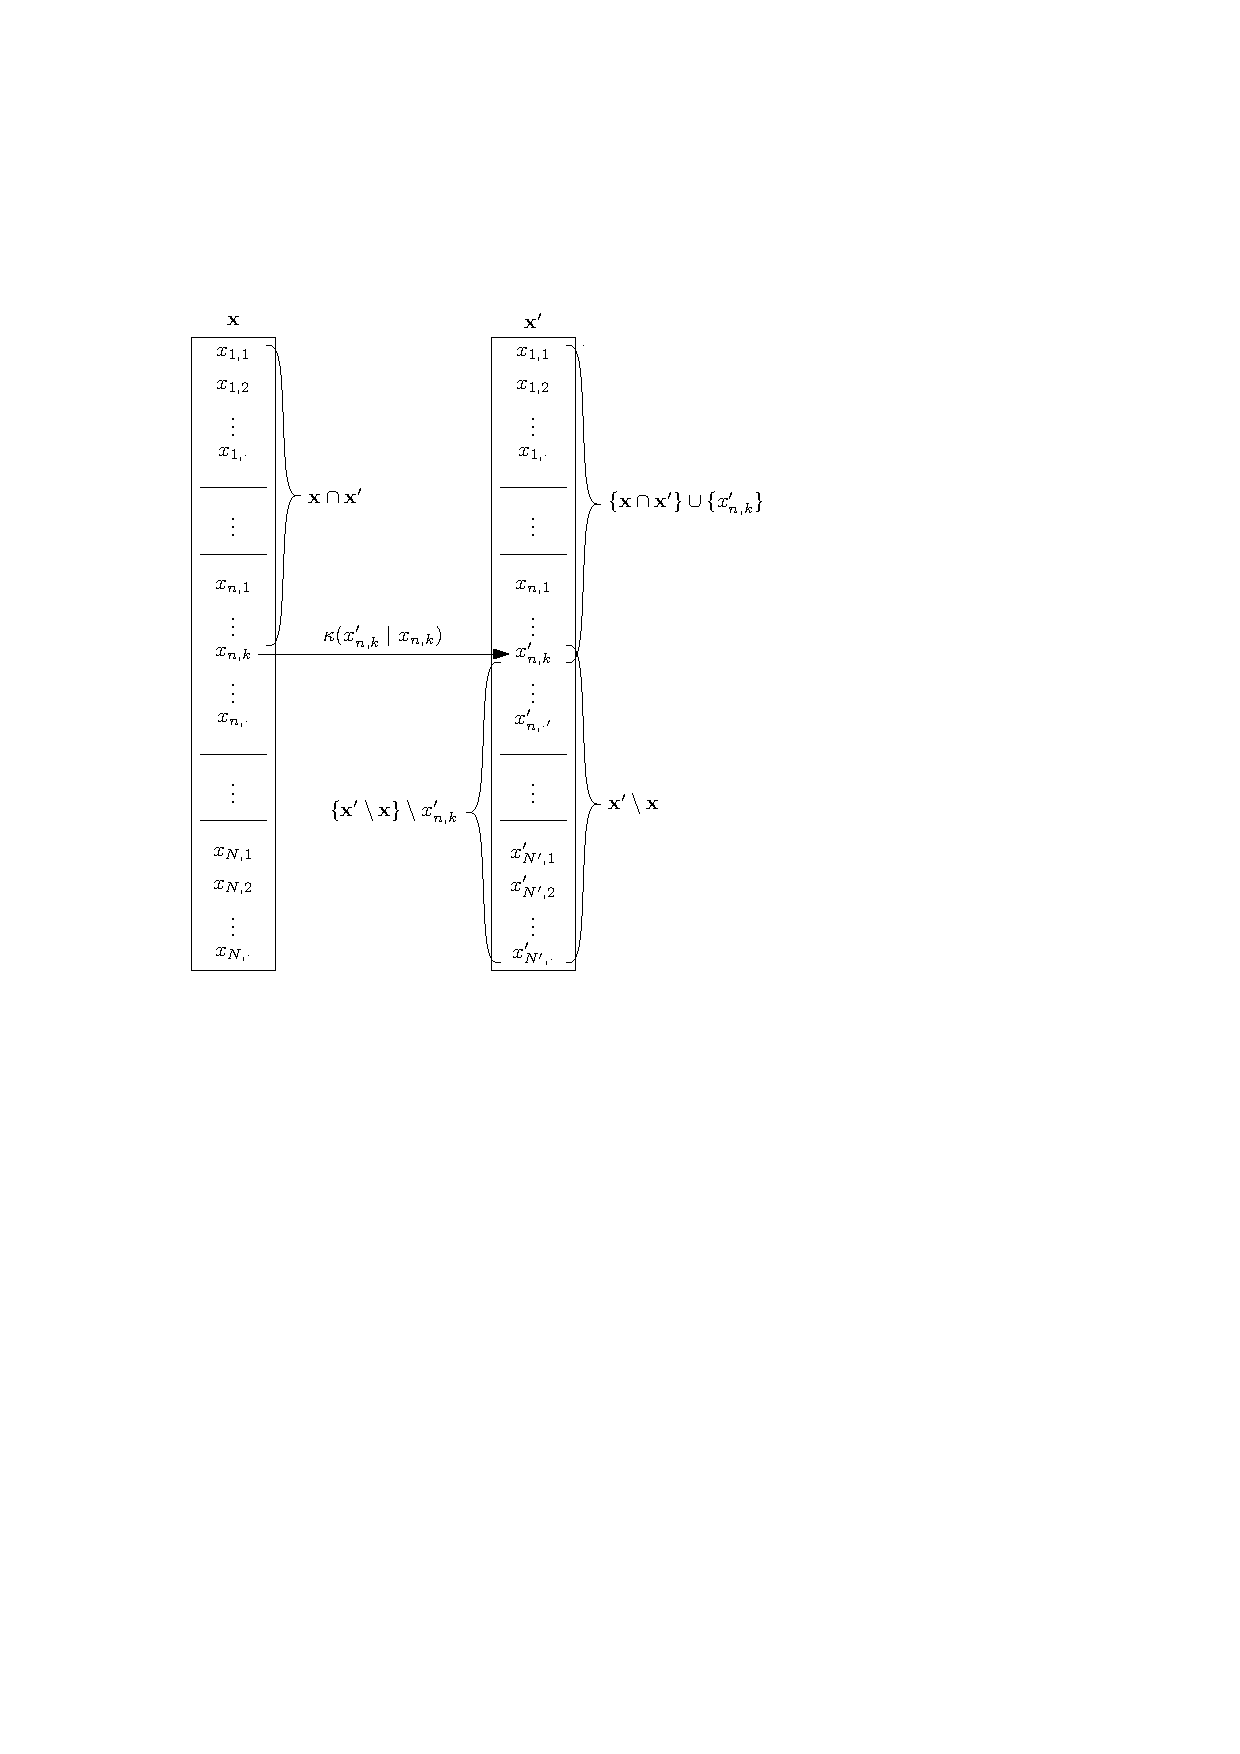
\includegraphics[scale=1]{pprog/how/figures/rdb/rdb}
\caption{Illustration of the RDB proposal step.}
\label{fig:pprog/how/figures/rdb}
\end{figure}
Following the Algorithm~\ref{alg:sampling/mcmc-mh/mh}, the proposal step consists of these steps:
\begin{itemize}
	\item Pick a single variable $x_{n, k}$ from the $|\vec x|$ random draws uniformly randomly.
	\item Get a new random choice $x'_{n, k}$ by sampling from a kernel $x'_{n, k} \sim \kappa(\cdot \mid x_{n, k})$. 
	\item Continue interpretation of program to get a new set of variables, $\vec x'$, that correspond to a new valid execution trace. (whenever a random procedure in the interpretation is the same as in $\vec x$, we reuse the existing value, only rescoring the conditional probability when necessary).
	\item $\vec x'$ is our MH proposal.
\end{itemize}
Following this procedure and notation in Figure~\ref{fig:pprog/how/figures/rdb}, the proposal distribution can be expressed as
\begin{equation}
	q(\vec x' \mid \vec x)	= \frac{\kappa(x'_{n, k} \mid x_{n, k})}{|\vec x|} \frac{p(\vec x' \setminus \vec x \mid \vec x' \cap \vec x)}{p(x'_{n, k} \mid \vec x' \cap \vec x)}
\end{equation}
The $1 / {|\vec x|}$ corresponds to randomly uniformly choosing a single variable. The $\kappa(x'_{n, k} \mid x_{n, k})$ corresponds to the proposal kernel. And finally,
\begin{align*}
	\frac{p(\vec x' \setminus \vec x \mid \vec x' \cap \vec x)}{p(x'_{n, k} \mid \vec x' \cap \vec x)}	&= p\left(\{\vec x' \setminus \vec x\} \setminus x'_{n, k} \mid x'_{n, k}, \vec x \cap \vec x'\right) \\
																										&= p\left(\{\vec x' \setminus \vec x\} \setminus x'_{n, k} \mid \{\vec x \cap \vec x'\} \cup \{x'_{n, k}\}\right) \\
\end{align*}
which corresponds to the probability of ``the rest of execution given the past random choices of this proposed execution trace''.

The acceptance probability can be written as
\begin{align}
	\mathcal A(\vec x' \mid \vec x)	&= \min\left(1, \frac{p(\vec y', \vec x') q(\vec y, \vec x \mid \vec y', \vec x')}{p(\vec y, \vec x) q(\vec y', \vec x' \mid \vec y, \vec x)}\right) \nonumber\\
									&= \min\left(1, \frac{p(\vec y \mid \vec x') p(\vec x') q(\vec x \mid \vec x')}{p(\vec y \mid \vec x) p(\vec x) q(\vec x' \mid \vec x)}\right) \label{eqn:pprog/how/rdb/acc}
\end{align}

In the \emph{propose from prior} case, a new random choice $x'_{n, k}$ is obtained by continuing the interpretation from $x_{n, k - 1}$ which means the expression of the kernel becomes $\kappa(x'_{n, k} \mid x_{n, k}) = p(x'_{n, k} \mid \vec x' \cap \vec x)$. Note that the reverse kernel becomes $\kappa(x_{n, k} \mid x'_{n, k}) = p(x_{n, k} \mid \vec x \cap \vec x')$. Hence the expressions for the proposal distribution (in both ways) become
\begin{align*}
	q(\vec x' \mid \vec x)	&= \frac{p(\vec x' \setminus \vec x \mid \vec x' \cap \vec x)}{|\vec x|} \\
	q(\vec x \mid \vec x')	&= \frac{p(\vec x \setminus \vec x' \mid \vec x \cap \vec x')}{|\vec x'|}
\end{align*}
Substituting this to the acceptance probability in \eqref{eqn:pprog/how/rdb/acc}, we obtain
\begin{equation}
	\mathcal A(\vec x' \mid \vec x) = \min\left(1, \frac{p(\vec y \mid \vec x') p(\vec x') |\vec x| p(\vec x \setminus \vec x' \mid \vec x \cap \vec x')}{p(\vec y \mid \vec x) p(\vec x) |\vec x'| p(\vec x' \setminus \vec x \mid \vec x' \cap \vec x)}\right)
\end{equation}

Summary: we just keep proposing and accepting and whenever a \verb!predict! is needed, we just report the current (or the corresponding function of a subset of) $\vec x$.